\documentclass[titlepage, 11pt]{report}
\usepackage[utf8]{inputenc}
\usepackage{a4wide}
\usepackage{graphicx}
\usepackage[toc,page]{appendix}
\usepackage[section]{placeins}
\usepackage{booktabs}
\usepackage{array}
\usepackage{hyperref}
\usepackage{natbib}
\usepackage{paralist}
\usepackage{fancyhdr}
\usepackage[toc,acronym,nogroupskip]{glossaries}

%%Some additional table column specifiers, allowing for fixed width columns that wrap.
\newcolumntype{L}[1]{>{\raggedright\let\newline\\\arraybackslash\hspace{0pt}}p{#1}}
\newcolumntype{C}[1]{>{\centering\let\newline\\\arraybackslash\hspace{0pt}}p{#1}}
\newcolumntype{R}[1]{>{\raggedleft\let\newline\\\arraybackslash\hspace{0pt}}p{#1}}

%%Fancy header!
\pagestyle{fancy}
\fancyhf{}
\fancyhead[L]{\leftmark}
\fancyfoot[C]{\thepage}
\setlength{\headheight}{14pt}

%%TOC up to subsubsection:
\setcounter{tocdepth}{2}

%%Glossaries setup
\chapter{Acronym List}

\begin{acronym}[AAAAA]
    \acro{cmm}[CMM]{Capability Maturity Model}
    \acro{cmmi}[CMMi]{Capability Maturity Model integration}
    \acro{7s}[7S]{Seven S model}
    \acro{rup}[RUP]{Rational Unified Process}
    \acro{scrum}[Scrum]{Scrum}
    \acro{yagni}[YAGNI]{You aren't gonna need it}
    \acro{sei}[SEI]{Software Engineering Institute}
    \acro{spa}[SPA]{The Spotify Approach}
    \acro{ac}[AC]{Agile Coach}
    \acro{po}[PO]{Product Owner}
    \acro{esa}[ESA]{European Space Agency}
    \acro{hood}[HOOD]{Hierarchic Object-Oriented Design}
    
    % CMMI core process areas
    
        % Level 2
        \acro{cm}[CM]{Configuration Management}
        \acro{ma}[MA]{Measurement and Analysis}
        \acro{sam}[SAM]{Supplier Agreement Management}
        \acro{pp}[PP]{Project Planning}
        \acro{pmc}[PMC]{Project Monitoring and Control}
        \acro{reqm}[REQM]{Requirements Management}
        \acro{ppqa}[PPQA]{Process and Product Quality Assurance}
        
        % Level 3
        \acro{dar}[DAR]{Decision Analysis and Resolution}
        \acro{ipm}[IPM]{Integrated Project Management}
        \acro{opd}[OPD]{Organisational Process Definition}
        \acro{opf}[OPF]{Organisational Process Focus}
        \acro{ot}[OT]{Organisational Training}
        \acro{rskm}[RSKM]{Risk Management}
        \acro{rd}[RD]{Requirements Development}
        \acro{ts}[TS]{Technical Solution}
        \acro{pi}[PI]{Product Integration}
        \acro{ver}[VER]{Verification}
        \acro{val}[VAL]{Validation}
        
        % Level 4
        \acro{opp}[OPP]{Organisational Process Performance}
        \acro{qpm}[QPM]{Quantitative Project Management}
        
        % Level 5
        \acro{car}[CAR]{Causal Analysis and Resolution}
        \acro{opm}[OPM]{Organisational Performance Management}
        
\end{acronym}
\makeglossaries
\newcommand{\ac}[1]{\gls{#1}}
\newcommand{\acs}[1]{\acrshort{#1}}
\newcommand{\acp}[1]{\glspl{#1}}

\title{Software Process -- Assignment 2\\
       \small ``Failure is always an option.''
}%really?
\author{Jelle van Assema 
  \and Felix Barten
  \and Robert Diebels
  \and Jasper Dijt
  \and Yoan-Alexander Grigorov
  \and Guido Loupias
  \and Edward Poot 
  \and Theologos Zacharopoulos
}
\date{\today}


\begin{document}
\maketitle
\tableofcontents{}
\chapter{Introduction}
Acronym test: \ac{rup} 

\ac{cmmi} 

\ac{7s}

\chapter{Capability Maturity Model Integration}

The \ac{cmmi} model is a model for evaluating the reliability of companies. The model contains guidelines for process improvement within an organisation. Since \ac{cmmi}'s inception there are more areas of business the model can be applied to: Production and development (\ac{cmmidev}), Service establishment (\ac{cmmisvc}) and Product and Service acquisition (\ac{cmmiacq})~\citep{ProductCMMIfor2010}.

The \ac{cmmi} model is the successor of the \ac{cmm} model which was developed between 1986 and 1993. The \ac{cmm} model originates from the software development world but is now often used in companies outside of the software business. The \ac{cmm} model was developed by the \ac{sei} by request of the US air force. The US Air force had difficulty finding contractors for their software projects and wanted a way find a way to identify reliable contractors.

\begin{figure}[!ht]
    \centering
        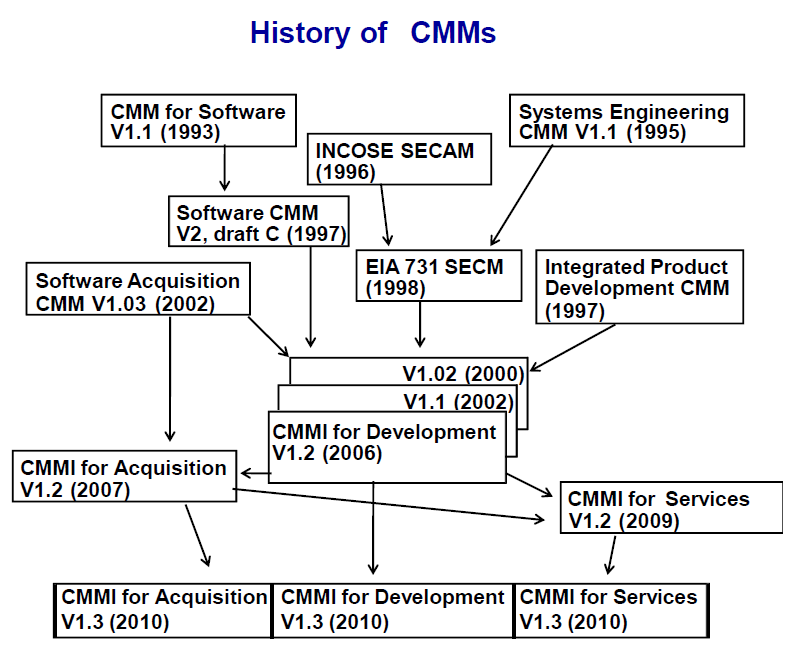
\includegraphics[width=0.6\textwidth]{graphics/cmmi_history}
    \caption{The History of \acp{cmm}}
    \label{fig:cmmi_history}
\end{figure}

\ac{cmmi} is often used when a company's reliability needs to be established, for example, with tender assignments. The \ac{cmmi} model has five levels of maturity an organisation can be assigned, with level five being the highest. \ac{cmmi} does not provide certifications for companies but rather appraises them at one of the five levels of \ac{cmmi}. All companies are automatically appraised at maturity level one of \ac{cmmi}. Companies are often appraised when they accept new contracts or when they want to measure how their production process is working compared to \ac{cmmi} best practices. If an organisation wants to increase its \ac{cmmi} maturity level there is no set amount of time that it will take. The process of raising the maturity level can take a month to many months depending on the commitment of the company~\citep{cmmifaq}. 

\section{The CMMi Model Framework}
% Needs REF.
The \ac{cmmi} model framework consist of the following core process areas:
%JWD: made more compact.
\begin{compactitem}
    \item \ac{car}
    \item \ac{cm}
    \item \ac{dar}
    \item \ac{ipm}
    \item \ac{ma}
    \item \ac{opd}
    \item \ac{opf}
    \item \ac{opm}
    \item \ac{opp}
    \item \ac{ot}
    \item \ac{pi}
    \item \ac{pmc}
    \item \ac{pp}
    \item \ac{ppqa}
    \item \ac{qpm}
    \item \ac{rd}
    \item \ac{reqm}
    \item \ac{rskm}
    \item \ac{sam}
    \item \ac{ts}
    \item \ac{val}
    \item \ac{ver}
\end{compactitem}

\section{Competence Areas in the Processes}
\ac{scrum}, \ac{rup} and the process followed by Ariane 5 will be judged on how well the core process areas are covered by these processes. 
This is done in table~\ref{tab:cmmi_l2} for level two, table~\ref{tab:cmmi_l3} for level three, table~\ref{tab:cmmi_l4} for level four, and table~\ref{tab:cmmi_l5} for level five. The following coverage levels are assigned to each process area for each process.

\noindent
\begin{tabular}{>{\bfseries}L{0,15\textwidth}L{0,85\textwidth}}
    High    & Fully covered by process used.\\
    Medium  & Partially covered by process used.\\
    Low     & Poorly covered by process used.\\
    None    & Not covered by process used.\\
    Unknown & Not enough information to determine level.\\
\end{tabular}

%\begin{compactdesc}
%\item[High] Fully covered by process used.
%\item[Medium] Partially covered by process used.
%\item[Low] Poorly covered by process used.
%\item[None] Not covered by process used.
%\item[Unknown] Not enough information to determine level.
%\end{compactdesc}
% Plan:
% - Set criteria to determine if competency applies to process

\begin{table}[ht!]
    \centering
    \begin{tabular}{>{\bfseries}l|*{7}{c}}
        Process     & \acs{cm} & \acs{ma} & \acs{pmc} & \acs{pp} & \acs{ppqa} & \acs{reqm} & \acs{sam}  \\
        \midrule
        RUP         & High & Medium & Medium & Medium & High & High & None \\ 
        Scrum       & Low & High & High & Low & Low & High & None \\ 
        Ariane 5    & Unknown & Low & Unknown & Low & Unknown & Unknown & Unknown \\ 
    \end{tabular}
    \caption{Maturity Level 2 - Managed}
    \label{tab:cmmi_l2}
\end{table}


\begin{table}[ht!]
    \centering
    \begin{tabular}{>{\bfseries}l|*{6}{c}}
        Process & \acs{dar} & \acs{ipm} & \acs{opd} & \acs{opf} & \acs{ot} & \acs{rskm} \\
        \midrule
        RUP     & None & Medium & None & None & None & Medium \\
        Scrum   & None & Medium & Low & Medium & None & Low \\ 
        Ariane 5 & Unknown & High & Unknown & Unknown & Unknown & Medium \\
    \end{tabular}
    \vspace{\baselineskip}\linebreak
    \begin{tabular}{>{\bfseries}l|*{5}{c}}
         Process & \acs{rd} & \acs{ts} & \acs{pi} & \acs{ver} & \acs{val} \\
         \midrule
         RUP & High & Medium & High & High & High \\ 
         Scrum & High & None & None & None & None \\ 
         Ariane 5 & Low & Unknown & Low & High & Medium \\ 
    \end{tabular}
    \caption{Maturity Level 3 - Defined}
    \label{tab:cmmi_l3}
\end{table}

\begin{table}[ht!]
    \centering
    \begin{tabular}{>{\bfseries}l|cc}
        Process & \acs{opp} & \acs{qpm} \\
        \midrule
        RUP     & None & Low \\   
        Scrum   & None & Low \\
        Ariane 5 & Unknown & Unknown \\
    \end{tabular}
    \caption{Maturity Level 4 - Quantitatively Managed}
    \label{tab:cmmi_l4}
\end{table}

\begin{table}[ht!]
    \centering
    \begin{tabular}{>{\bfseries}l|cc}
        Process & \acs{car} & \acs{opm} \\
        \midrule
        RUP     & Low & None \\
        Scrum   & Medium & Low \\
        Ariane 5 & High & Unknown \\
    \end{tabular}
    \caption{Maturity Level 5 - Optimising}
    \label{tab:cmmi_l5}
\end{table}


\FloatBarrier
\subsection{RUP}

As it is mentioned in the '\ac{cmmi} for developers' document~\citep{team2010cmmi}, \ac{cmmi} itself is not a process description, but instead it describes characteristics (process areas) of a good software process. Additionally, it is a map that identifies gaps in existing processes that may need to be filled. 
On the other hand, \ac{rup} is an iterative software process which maps to many \ac{cmmi} process areas. 
While \ac{cmmi} describes the ``what'', \ac{rup} describes the ``how''. 
The synergy between those two addresses any gaps they collectively define and eliminates redundancy. 
As it can be seen from the table and as Gallagher et al.~\citep{gallagher2001rational} conclude; \ac{rup} maps some parts \ac{cmmi} in it's workflows and activities.

\subsubsection{Maturity Level 2}
Firstly, analysing the \textbf{\textit{Maturity Level 2}} process area, \ac{cm} is present in \ac{rup} as a specific artifact, including an established \ac{cm} system, tracking and controlling changes, and configuration audits.

\ac{ma} is not defined solely in \ac{rup}; there is no description on details or metrics and analytics definition. However, the definition includes measurements specification, analysis reports, results and communicative data.

\ac{pmc} in \ac{rup} has some some incompatibilities, while \ac{rup} monitors areas such as project planning, risks, stakeholders, progress and milestones, it has problems on commitments monitoring and data management. Also, \ac{rup}'s corrective actions are explicit and include issues management and corrective actions management.

Furthermore, \ac{pp} is slightly supported by \ac{rup} since it includes definitions of the project size, efforts and cost estimation and risks identification. But it does not support project attributes estimation, data management and project resources planning. 

\ac{ppqa} is mapped by \ac{rup} owning to the support of evaluation of the processes, products and services.
The mapping of \ac{reqm} and \ac{rup} is also clear because in \ac{rup} the inception phase consists of of a set of requirements analysis including commitment, support of changes and support of later requirements refinements. 

Last element of this process area is the \ac{sam}. \ac{rup} has no support on this area since it is not defined at all.

\subsubsection{Maturity Level 3}
Secondly, in case of the \textbf{\textit{Maturity Level 3}} process area \ac{dar}, \ac{opd}, \ac{opf} and \ac{ot} are not defined in \ac{rup} and are not supported inside the scope of \ac{rup}. However, \ac{ipm} has a few points which can be mapped in \ac{rup}, including the integrated plans in project management, issues resolving and stakeholders involvement management. In addition to that, \ac{rup} slightly supports integrated plans and project process establishment but no dependencies management.

\ac{rup} is a risk-first process by including risk identification, classification and prioritisation. However, what \ac{rup} misses is a risk parameters definition and an explicit risk management strategy (\ac{rskm}).

The development, validation and analysis of the requirements (\ac{rd}) in \ac{rup} is a very explicit process. From the customer perspective, during the inception phase, there is requirements elicitation, stakeholders need collection and  translation of stakeholders needs to customer requirements. On the product requirements side, there is explicit product establishment identification.

\ac{ts} is addressed by \ac{rup} since the process is very specific in development and design, it suggests effective design methods, comprehensive interfaces and interfaces descriptions establishment. However, the selection of product component solutions is missing from \ac{rup} because it does not mention detailed alternative solutions development, but the evolution of operational concepts and scenarios are clearly stated.

\ac{pi} in \ac{rup} is established by \textit{product integration strategies} and \textit{environments}, interfaces management, and finally, explicit component integration and product deployment procedures.

Both \ac{ver} and \ac{val} are established by specific practices of \ac{rup}. First, for verification \ac{rup} includes a verification strategy and environment, including peer reviews and analyses of review data. Second, for validation, it also includes validation strategy and environment. Additionally for both cases data gathering and analysis is included for continuous improvement.

\subsubsection{Maturity Level 4}
Thirdly, \textbf{\textit{Maturity Level 4}} process area includes \ac{opp} which is not defined in the scope of \ac{rup} and \ac{qpm} which is it can be slightly mapped in the composition of the defined process that \ac{rup} supports.

\subsubsection{Maturity Level 5}
Finally, in \textbf{\textit{Maturity Level 5}} process area, \ac{car} can be slightly mapped in \ac{rup} in terms of analysis data selection support and changes evaluation. No data records are kept after the end of every phase and no metrics extracted.
However, \ac{opm} is something that is not mentioned in \ac{rup}.

\subsection{Scrum}
\subsubsection{Maturity Level 2}
When we dive into analysing \textbf{\textit{Maturity Level 2}} for the Scrum framework we are able to conclude that a lot of process areas are well covered. 

However, if we look into \ac{cm} area it is easy to point out that Scrum is not always that specific. In fact, for \ac{cm} only the User Stories are described by Scrum. 

Furthermore, it is easy to conclude that \ac{ma} is highly covered within Scrum. Simply put, the Scrum Master has the sole responsibility to maintain the Scrum framework implementation itself \citep{schwaber2011scrum}. 

The \ac{pmc} is also recognised as a strong area in Scrum. As the framework is focuses on delivery, Scrum includes useful practices for project monitoring and control. Moreover, Scrum integrates the Sprint Planning, Daily Scrum, Sprint, Sprint Review and the Sprint Retrospective in order to accomplish successful control over the work, and monitoring over the separate development steps. Furthermore, the Sprint Planning and the Sprint Review are greatly influencing the success in the \ac{pp} area. 

In addition, the Product Owner role is responsible for interacting with relevant stakeholders appropriately, and giving guidance to the Development Team in terms of business requirements. However, Scrum is not very specific about quality assurance. The Definition of "Done" is agreed within the team and the process itself is not definite enough about the \ac{ppqa}. 

Since all the business requirements are covered specifically by the Product Owner, Scrum has a dedicated role. Therefore the \ac{reqm} area is also well covered. 

Last but not least, \ac{sam} is not described in Scrum.

\subsubsection{Maturity Level 3}
In contrast to the previous level, \textbf{\textit{Maturity Level 3}} is not so well defined within the \ac{scrum} framework. Process areas such as \ac{dar}, \ac{ot}, \ac{ts}, \ac{pi}, \ac{ver} and \ac{val} are not described in \ac{scrum}.

However, the \ac{rd} area is implemented within the Scrum framework with the usage of Sprint Planning meetings, Sprint Reviews and Sprint Retrospectives.

Furthermore, the \ac{ipm} is expressed in \ac{scrum} by the Increment \citep{schwaber2011scrum}, the Scrum Retrospective, and the Scrum of Scrums \citep{sutherland2001inventing}. Simply put, the Increment can be used to estimate time-frames better, the Scrum Retrospective to learn from mistakes made during the Sprint and the Scrum of Scrums to spread lessons throughout the entire organization. The Scrum Retrospective and the Scrum of Scrums also collaborate for having a medium state of \ac{opf}. The Scrum of Scrums in particular also gives the framework a glimpse of what \ac{opd} is.

Finally, we have the \ac{rskm} which is not specifically expressed within Scrum. As Scrum is focused generally on product delivery, the risk management is limited only to technical risks. In fact, even the technical risk management is dependent on the definition of "Done" \citep{schwaber2011scrum}.

\subsubsection{Maturity Level 4}
The \ac{opp} is not maintained within \ac{scrum}. However, the \ac{qpm} is somehow supported mainly because of the Increment \citep[page 15]{schwaber2011scrum}. Generally speaking, the Increment can provide statistical data for the project’s objectives for quality and process performance.

\subsubsection{Maturity Level 5}
The \ac{car} process area is partially supported within Scrum. In general, identifying and analysing causes of problems is done in the Sprint Retrospective. Furthermore, the purpose of the Sprint Retrospective is to address the issues founds and to make sure that they are not going to appear again \citep[page 12]{schwaber2011scrum}. However, \ac{scrum} is not so specific in how exactly those actions are taken. Moreover, it is unspecified what are the approaches towards technical problems, design issues, testing failures, etc. 

Furthermore, the \ac{opm} has some characteristics maintained in \ac{scrum}. In general, the product and process quality can be increased by implementing Sprint Retrospectives. In addition, the process implementation itself is maintained by the Scrum Master. However, \ac{scrum} does not define steps to decrease Sprint time-frames, how exactly product quality is improved, and how to shorten out the time required to change/maintain functionality.

% ========
% Ariane 5
\subsection{Ariane 5}
This subsection is meant to analyse the failed case we chose during Assignment 1 of the Software Process course.
We will be assessing to what extent the organisational process for the development of the Ariane 5 rocket fits the \ac{cmmi} model. \ac{esa} has standards \citep{esaSEstandards1991} which are surprisingly similar to \ac{cmmi}. They range from project management to actual verification and validation of software. We split up each \ac{cmmi} project area into what the \ac{esa} standards describe and what we actually know happened in the case.

\subsubsection{Maturity Level 2}
We begin with assessing compliance to \textbf{\textit{Maturity Level 2}}.

\begin{description}
\item[\ac{cm}]
\ac{esa} defines a specific procedure for software configuration management \citep[82]{esaSEstandards1991}. They mention several activities to be performed for \ac{cm}. Ranging from \textit{configuration identification} to \textit{configuration status accounting}. They specify what should happen during a release and what should happened to old release and state that all activity related to \ac{cm} should be recorded in a \textit{software configuration management plan} We can assess that the \ac{esa} standards for \ac{cm} are \textit{high}.

 We know that the process is spread across a multitude of companies. This would indicate that there has to be some form of \ac{cm} in order to manage code configurations and releases. As mentioned the \ac{esa} standards specify that there has to be a   However actual information concerning \ac{cm} in the Ariane case is \textit{unknown} to us. 

\item[\ac{ma}]
\citep[38]{esaSEstandards1991} specify that: "Where appropriate, software quality attributes should be specified in measurable terms (i.e. with the use of metrics).". They do not state \textit{how} this should be done. There are further mentions of analysis and measurement on \citep[46]{esaSEstandards1991} during the architectural design phase, verification and validation \citep[95]{esaSEstandards1991}. So we can conclude that the \ac{esa} standards with respect to \ac{ma} is \textit{high}.

\ac{ma} assesses the compliance of an organisations' process in order to quantify aspects that belong to it. In terms of software development this would equal to testing and software metrics. What we know from the Ariane case is that one of the problems that was identified concerned inadequate testing. Information concerning software metrics is \textit{unknown} to us. This would mean that compliance with \ac{ma} is \textit{low} at best. 

\item[\ac{pmc}]
\ac{esa} standards provide no specific chapter on project monitoring and control. Though chapters describing requirements, reference to cost estimates and project monitoring are made. 
No specific implementations are suggested other than the fact that estimates and monitoring should be present in the relevant plans.
This would lead us to conclude that the \ac{esa} standards are \textit{medium} as specifics on cost monitoring are nowhere to be found.

Due to a lack of relevant information compliance to \ac{pmc} for the failed case is \textit{unknown} to us. 

\item[\ac{ppqa}]
The \ac{esa} standards specify that it should be clear \textit{how} software quality is achieved. Experts are free to choose their own quality implementations as long as they document how this is done in the \textit{software quality assurance plan}. This plan is almost linear to what the \ac{ppqa} phase in \ac{cmmi} want to capture. This leads us to conclude that \ac{ppqa} compliance for the standards is \textit{high}.

Concerning compliance to \ac{ppqa} for the failed case, some evaluations \citep{monfort1996ariane}, \citep{denskat1996development}, show that the programming language Ada had specific pitfalls developing for certain targets (processors). We have seen no evidence that these evaluations were used during the process. This does not mean that this was not the case. Considering this information we would assess compliance as \textit{low}. However as we do not have any information concerning the  processes in place, we will state that compliance to \ac{ppqa} for the failed case is \textit{unknown} to us.

\item[\ac{dar}]
\ac{esa} standards provide two distinct phases for the assessment of requirements, the \ac{ur} phase and the \ac{sr} phase. For instance, how to deal with requirements change, how to classify user requirements and how to specify software requirements. We would assess that the compliance with \ac{reqm} for the \ac{esa} standards is \textit{high}.

Compliance to \ac{reqm} for the failed case is \textit{unknown} to us. 

\item[\ac{sam}]
Regarding \ac{sam} and the \ac{esa} standards there is a specific mention that\citep[510]{esaSEstandards1991}:  "Software items acquired from external suppliers must always be checked against the standards for the project.". Furthermore it is stated that: "An SQAP shall be produced by each contractor developing software. An SQAP is not required for commercial software.".
Making each supplier obligated to conduct quality assurance according to \ac{esa} standards.
We conclude that compliance to \ac{sam} is \textit{high}.

Compliance to \ac{sam} is \textit{unknown} to us. We do have information concerning the amount of prime-contractors (which was Airbus Space and Defense) and sub-contractors for the Ariane case. Though information on how the suppliers are managed is not known.

\end{description}

\subsubsection{Maturity Level 3}
Compliance to \textbf{\textit{Maturity Level 3}} is described below.

\begin{description}
\item[\ac{dar}]
Concerning \ac{dar} the \ac{esa} standards require that decisions made during code reviews be documented in a \ac{rid}. They go on to state that \citep[44]{esaSEstandards1991}: "Design decisions should be recorded." in regard to software design, so not just code reviews are documented.
We conclude that the \ac{esa} standards compliance with \ac{dar} is \textit{medium} as they do not specify whether alternatives should be provided, or what happens to the decisions after they are documented.

We have insufficient information to assess compliance to \ac{dar}. We do know that decisions were made about a testing vs. performance trade-off consistently. However, we were unable to find the decision documentation for this case. We conclude that the compliance for the failed case is \textit{unknown} despite this information. 

\item[\ac{ipm}]
\ac{esa} adheres to the \ac{ipm} process area by providing a multitude of standards for software and projects to apply. This creates integration within all projects. Just as it requires suppliers to create software quality assurance plans.
We assess that for \ac{esa} standards this process area is \textit{high}.

Compliance to \ac{ipm} is \textit{high}. We know that \ac{esa} had defined a multitude of processes for project management. These were established as early as 1982 when \ac{esa} commissioned the HOOD methodology for managing software within the project. We know that these processes where in use during the failure of the case.

\item[\ac{opf}]
The \ac{esa} standards make no mention of process improvements specifically. Aside from recommended improvements for during software validation. We therefore assess that the compliance within the \ac{esa} standards for \ac{opf} is \textit{low}.

Compliance for the failed case to \ac{opf} is \textit{unknown} to us. 

\item[\ac{opd}]
Regarding \ac{cmmi}'s \ac{opd} area, \ac{esa} is quite clear, \citep[22]{esaSEstandards1991}: " A life cycle approach, based upon this model, should be defined, for each project, in the Software Project Management Plan.". They suggest three specific organisational definitions: Waterfall, incremental, evolutionary. Along with the disadvantages that are part of them. Like \ac{cmmi} they do not specify which one to use. We conclude that for the standards the compliance with \ac{opd} is \textit{high}.

Compliance for the failed case to \ac{opd} is \textit{unknown} to us. Information we do have suggests usage of a Waterfall-esque method. 

\item[\ac{ot}]
Considering \ac{ot} compliance with the \ac{esa} standards we find that \ac{esa} mentions staff training and experience as a \textit{risk area} \citep[76]{esaSEstandards1991}. Further emphasis is placed on adequate training of personnel when assessing software quality. Suggested training for personnell would have to be documented in the \textit{Software Project Management Plan}.
We would assess \ac{esa} compliance withe \ac{ot} to be \textit{medium}. As it is not explicitly mention that it \textit{must} be done.

Compliance to \ac{ot} during the time our case was relevant is \textit{unknown}. According to \citep{esatraining2016} \ac{esa} currently does offer training programmes. 

\item[\ac{rskm}]
The \ac{esa} standards specify \ac{rskm} within two of the management standards. \textit{Software project management} and \textit{software quality assurance} they mention several potential risk areas though they don't go into specifics. \ac{esa} standards only state that the potential risks \textbf{should} be identified so that they can be contained.

Compliance to \ac{rskm} for the failed case we assess as \textit{medium}. This is due to papers/articles such as \citep{nuseibeh1997ariane}. Where they state that inadequate risk-management played a significant role in the failure of the case.

\item[\ac{rd}]
\ac{rd} within the \ac{esa} standards is highly emphasised. There are two specific phases dedicated to requirements development as mentioned before. How to specify requirements is document and other related matters are specified.

Compliance with \ac{rd} is \textit{low}. One of the prime causes for the failure of the Ariane 5 case was that code from the Ariane 4 had been re-used. This code had different requirements. Proper implementation of \ac{rd} might have prevented the failure.

\item[\ac{ts}]
Concerning \ac{esa} standards and \ac{ts} we can immediately conclude that the standards are almost a direct copy of this process area. The standards focus on providing a framework instead of forcing the engineers to adopt a certain solution. 
We assess that \ac{ts} compliance is \textit{high}.

Compliance with \ac{ts} for the failed case is \textit{unknown} to us. Information concerning alternative solutions provided to technical problems are unavailable to us. Furthermore implementation details for technical solutions are not enforced by \ac{cmmi}, so \ac{esa} was free in their implementation.

\item[\ac{pi}]
\ac{esa} standards show some concern of integration testing for a multitude of components. They state that \citep[51]{esaSEstandards1991}: "Integration test plans must be defined in the integration test section of the Software Verification and Validation Plan". This means that it is an obligation to specify integration test tactics. Further mention is made of integrating other products, though not specifically as a risk area.
We can conclude that \ac{pi} compliance according to the standards is \textit{medium}.

Compliance with \ac{pi} structure was \textit{low} for the failed case. One of the problems we identified during Assignment 1 was that integration of software components was difficult. This resulted in days being set aside for component integration.

\item[\ac{ver}]
\ac{esa} standards specify what should be done during software verification in a separate chapter. Aside from that verification is mentioned through out the standards ranging from Architectural design verification and what means exist to conduct verification.
We would assess compliance with \ac{ver} to be \textit{high}.

Compliance with \ac{ver} for the failed case is \textit{high}. \ac{esa} has a committee, \citep{esastandardizationBSSC} dedicated to standardisation and software engineering. They determine the standards for software with \ac{esa}. Evidently this didn't stop the failure in the Ariane case. From a \ac{cmmi} perspective \ac{esa} fits the bill.

\item[\ac{val}]
Similar to \ac{val} validation of correctness of the software is mentioned throughout the document. It shares a chapter with verification as the two are closely related.
Verification and validation decisions/requirements are placed in a \textit{Software Verification and Validation Plan} for a full overview concerning this topic.
We would assess compliance with \ac{val} for the \ac{esa} standards to be \textit{high}.

Compliance with \ac{val} for the failed case is \textit{medium}. The Ariane case showed several instances of validation failures, which led to the failure. However rigorous testing/validation methods were in place to ensure the right product was being build. This means that at the time of the failure the rating would be \textit{medium}.

\end{description}

\subsubsection{Maturity Level 4}
Compliance to \textbf{\textit{Maturity Level 4}} is described below. 

\begin{description}
\item[\ac{opp}]
The \ac{esa} standards make no mention of evaluations concerning improvements of the processes used or the standards themselves. We know that the standards get revised every couple of years as is seen in the document history. However, any specification concerning process improvement is non-existent.
We assess the standards to have \textit{no} explicit compliance to \ac{opp}.

Compliance to \ac{opp} for the failed case is \textit{unknown} to us. In our research for this case we were unable to find any quantitative assessments performed by the organisation themselves before the failure. 

\item[\ac{qpm}]
\ac{esa} standards specify no means or measurements in order to quantify process management. They have vague statements about cost estimations having to be accurate to 30\% \citep[42]{esaSEstandards1991}. Compared to what? The standards don't mention any other quantitative measures for project management.
So we conclude that compliance with \ac{qpm} is \textit{low}.

Compliance to \ac{qpm} at the moment of failure is \textit{unknown} to us. Currently is it known to us that \ac{esa} has developed a project management tool that addresses/quantifies project management \citep{esapmgmnt2016}.

\end{description}

\subsubsection{Maturity Level 5}
Compliance to \textbf{\textit{Maturity Level 5}} is described below. 

\begin{description}

\item[\ac{car}]
The standards make no mention of what should happen in the event of a failed project. Though as seen previously, documentation according to the standards should be extensive.
Leading us to conclude that the compliance to \ac{car} is at least \textit{medium}.

Compliance to \ac{car} for the failed case is \textit{high}. In the Ariane case extensive research has been done in order to learn as much as possible from the failure and prevent future failures. 

\item[\ac{opm}]
\ac{esa} standards mention nothing concerning active improvement of standards or processes. Whether this means they are not looking for process management improvement is unclear to us.
So we mark compliance to \ac{opm} as \textit{unknown}.

Compliance to \ac{opm} for the failed case is \textit{unknown} to us. We have found several examples where \ac{esa} requests feedback to improve performance. Though they are current-day examples, concerning the time-period of the failure little information is available.

\end{description}

\section{Planning \& Predictability}
This section is intended to provide a more in-depth view from a Planning \& Predictability perspective. How do Scrum and \ac{rup} handle planning? Do they even plan ahead? What about the Ariane case? We will study these questions and try to extract any valuable lessons.

\subsection{Scrum}
\ac{scrum} is an iterative process which focuses on scheduled product delivery \citep{schwaber2011scrum}. In conjunction with \ac{cmmi} we can observe how process areas are expressed within the framework. Generally speaking, on management and defined levels we have partial implementation.
However, the delivery focused nature of \ac{scrum} stands out when \ac{cmmi} is drawn.

When we pick \acrlong{pp} and investigate its correlation with \ac{scrum} we can easily notice an interesting parallel between what \ac{cmmi} requires at a project level in general, and what \ac{scrum} defines as practises during a Sprint.

\subsubsection{Project Estimations}

The first specific goal of the \ac{pp} is to establish project estimations. More specifically, this topic is divided into project scope estimation, work product/task attributes estimation, project lifecycle phases estimation, and lastly cost and effort estimations \citep[page 283]{team2010cmmi}. In parallel, \ac{scrum} sums a lot of those goals within the Sprint Planning. Moreover, the \acrfull{wbs} is very similar to resolving the difficulty and priority of Product Backlog items \citep[page 283]{team2010cmmi}:

\begin{quote}
The \ac{wbs} evolves with the project. A top-level \ac{wbs} can serve to structure initial estimating. The development of a \ac{wbs} divides the overall project into an interconnected set of manageable components.
Typically, the WBS is a product, work product, or task oriented structure that provides a scheme for identifying and organising the logical units of work to be managed, which are called “work packages.” 
\end{quote}

Furthermore, the project scope estimation includes the following routines \citep[page 284]{team2010cmmi}:

\begin{compactitem}
    \item Developing the \ac{wbs}
    \item Define work packages with specified estimations
    \item Identifying products and product components to be externally acquired
    \item Recognize reusable work products
\end{compactitem}

In contrast, the Sprint Planning establishes more of an abstract approach towards these goals. It is obvious that the \ac{cmmi} evaluation is significantly more specific. However, a parallel between the two is still possible. Mainly because of the major idea, which is estimation over tasks. 

Furthermore, the attributes estimation evaluates the process for size, level, connectivity, complexity, availability, and structure within the discussed project model \citep[page 284]{team2010cmmi}. Similarly to those goals, \ac{scrum} also addresses those task attributes during the Sprint Planning. 

Next is the project lifecycle estimation. In \ac{scrum} the team decides upon considerably small tasks compared to the \acs{cmmi} requirements. In \acs{pp} description the process is required to make a deep and detailed estimation over what seems to be a waterfall-like planning. 

Last in the project estimations is the overall cost and effort. Such correlation is not available within the \ac{scrum} framework practises.

\subsubsection{Developing Project Plan}
The developing of project plan sub-goal is again reflected by the Sprint Planning. During the plan meeting the Scrum team identifies Backlog Items difficulty level, divide the tasks, and breakdown the major concerns about listed requirements. 

Moreover, the \acs{cmmi} developing of project plan area consists of budget and schedule estimations, project's risk recognition, data management plan, project's resources plan, required knowledge and skills plan, stakeholder involvement plan, and project plan establishment. 

First, \ac{scrum} does not compliment any budget discussions. Secondly, project's risk recognition is part of the Sprint Planning. However, since the \ac{scrum} team is empowered and self-organized, there are no guidelines to what actually \textit{risk} is within the context of \ac{scrum}. Thirdly, the data management area is related to documents warehousing, and \ac{scrum} is silent towards this. Next we see that \ac{cmmi} is concentrating on precise evaluation of resources management with the resources planning \citep[page 293]{team2010cmmi}. The last three areas (plans for knowledge and skills, stakeholder involvement, and project establishment control) can be recognised within responsibilities of some fundamental \ac{scrum} principles and roles. Simply put, the \ac{scrum} team is meant to be composed by professionals \citep[page 5]{schwaber2011scrum}. Secondly, the stakeholders involvement is represented by the Product Owner. And last but not least, the Scrum Master's responsibility is to make sure that the process is followed and to fix where practises are going in blocking direction \citep[page 6]{schwaber2011scrum}.

In addition, the Product Owner has the sole responsibility to take care of the Product Backlog and to express stakeholders requirements clearly. Furthermore, during the entire Sprint the Product Owner's responsibility is to make sure that the Development Team understands the business idea behind what they are meant to implement.

\subsubsection{Obtain Commitment to the Plan}

Lastly, the \ac{pp} defines the \textit{Obtain Commitment to the Plan} point. In parallel, in \ac{scrum} a successful Sprint is a Sprint that has all tasks in its Sprint Backlog marked as \textit{Done}. In the \ac{scrum} community there are two types of Sprint Planning known: \textit{Velocity-driven sprint planning} and \textit{Commitment-driven sprint planning} \citep{www:www.mountaingoatsoftware.com}. Simply put, the commitment-driven approach first ensures that the top-priority tasks are selected for the upcoming Sprint, and secondly that the developers working on the tasks are committed to complete them. 

\subsubsection{Conclusion}
We can conclude that a number of goals from \acrlong{pp} in \ac{cmmi} can be met by the Sprint Planning event in \ac{scrum}. 
Initially, Product Item estimations are made during the Sprint Planning, similarly to the \acs{pp} in \ac{cmmi} for the whole project. In addition, developing project plan highlights stakeholders involvement which is typically represented by the Product Owner in \ac{scrum}. Furthermore, there is a clear correlation between obtaining plan commitment sub-goal and the Commitment-driven sprint planning. And finally, even though the \acrlong{pp} is more oriented into waterfall-style processes \citep[page 4]{gallagher2001rational}, the Sprint Planning event covers a lot of the specific goals within \ac{pp}.


% ========
% Rup 
\subsection{RUP}

% Rup insights Intro
By looking more into the \textit{planning} aspect we can argue that, \ac{rup}'s \textit{Business modelling} discipline, \textit{Project management} and \textit{Environment} supporting workflows / disciplines~\citep{kruchten2004rational}, map most of the specific goals of \ac{cmmi}'s \ac{pp} project area. In detail, \textit{Business modelling} refers to financial forecast, business objectives and intended market for the product. Additionally, \textit{Project management} supporting disciple refers to two levels of planning, the project planning and iteration planning \cite{west2002planning}. Finally, the \textit{Environment} focuses on the activities required to provide software development environment, including processes and tools. 

% First specific goal
\subsubsection{Project Estimations}
In order to address, first specific goal that is to ``establish estimates for attributes of the work products and tasks, and project cycle definition and costs'', we can look into the \textit{Project management} supporting disciple. As this discipline describes, the project planning takes place during the \textit{inception} phase and focuses specifically on the understanding of the ``scope'' of the project by planning phases and iterations. The deliverable of this phase is the scope of the project and the project life cycle (iterations and phases). Additionally, according to the \textit{Business modelling} discipline of \ac{rup}, a financial forecast including projected revenues and costs of the project should be determined. Meaning that \ac{cmmi}'s specific sub-goal of estimates of efforts and costs is also, covered. However, estimates of project attributes such task duration, resources, inputs, and outputs, are not addressed easily by \ac{rup}. \ac{rup} integrates those attributes during the iterations when the clear definition of implementation tasks is done. Although, a rough estimation take place during \textit{Business modelling} in order to assess the cost of the resources, the detailed estimation is not occur until the implementation phase starts.

% Second specific goal
\subsubsection{Developing Project Plan}
Next, the specific goal of ``plan development'', includes some sub-goals that are addressed explicitly in \ac{rup}. Firstly, the establishment of a budget is well defined by the \textit{Business modelling} discipline, which is it's purpose. Secondly, the project risk identification is one of the primary properties of \ac{rup} since it's a risk-driven process and risk-management is integrated into the development process. The establishment of the project plan, knowledge and skills, and stakeholder involvement is realised during the \textit{inception phase} according to the \textit{Project management} discipline. What's missing though, is a plan for the data management which is not uniquely addressed by any of the \ac{rup} artifacts. Additionally, the project resources planning is something that is also, missing from \ac{rup}. As it is mention above, \textit{Business modelling} discipline deals with it in a initial phase but iteration redefine it during the project's progress.

% Third specific goal
\subsubsection{Obtain Commitment to the Plan}
Finally, the specific goal of ``plan commitment'', is something that \ac{rup} defines during the \textit{inception phase}. This phase is not complete if the team and the stakeholders have not ``commit'' to a specific plan and any subordinate plans. Moreover, according to \citep{team2010cmmi} the ``reconcile work and resource levels'' sub-goal is typically accomplished by lowering or deferring technical performance requirements, negotiating more resources, finding ways to increase productivity, outsourcing, adjusting the staff skill mix, or revising all plans that affect the project or schedules. 
This is something that can be addressed by the \textit{Project management} discipline by making plans on how this should work. But mainly this is something that the \textit{Environment} discipline would address by providing tools and process that work in such circumstances. However, there is not solely statement in \ac{rup} to address these issues. 

\subsubsection{Rup and Project Management}
% Rup insights summary
As it can be seen, \textit{Project Management} supporting discipline, can be considered a useful workflow for risk management, monitoring and planning in a iteration level, however, this discipline does not attempt to cover all aspects of project management. From our point of view, in one hand \ac{pp} in \ac{cmmi} has a waterfall-like approach \citep{gallagher2001rational}, with more formal analysis of requirements and stakeholders, costs and risks, data and resources, and finally, knowledge and skills. On the other hand, \ac{rup} provides a \textit{medium} synergy with it, mainly because of attributes of the \textit{inception} phase, \textit{Project Management}, \textit{Business modelling} and \textit{environment} disciples. However, some parts are not explicitly defined during the planing, but they may be introduced in later phases and elaborate on previous issues, providing knowledge for the next iteration.

\subsubsection{Conclusion}
% Rup Conclusion
\ac{rup} is an adaptable process framework which incorporates many building blocks and makes explicit life-cycle phases with well defined deliverables. 
\ac{cmmi} is a process framework which also defines explicit processes and deliverables for every phase. For this reason, \ac{rup} and \ac{cmmi} complement each other in achieving a mature software organisation in many levels. However, there are some parts that \ac{rup} does not incorporate since they are more of the organisation side and not in the software process side. Thats the reason, \ac{rup} and \ac{cmmi} complement each other. 

% ========
% Ariane 5
%%Really need to restructure this. We found? I found?
\subsection{Ariane 5}
\subsubsection{Project planning or Improvement?}
If we look at the Ariane case from a project planning perspective we see that the \ac{esa} standards are actually quite smiliar to the \ac{cmmi} approach.
Like \ac{cmmi}, emphasis is placed on recording the entire process management procedure in a project plan. With a focus on reporting progress, planning and estimation of project costs. This is meant to increase the predictability of the project using terms similar to those mentioned by \ac{cmmi}.

What is striking about this is that if we would give the \ac{esa} standards a \ac{cmmi} level we would probably be near a maturity level of 4 or 5. Though comparing this to what happened during the actual failure, where specific implementations are either \textit{unknown} or \textit{low}, we see a big contrast.

With all the emphasis the standards place on planning and documentation, could a high \ac{cmmi} maturity level be a decent indicator? Or could full compliance with \ac{cmmi} have prevented the failure? 

Because of the striking similarity of \ac{cmmi} and the \ac{esa} standards we find this doubtful to say the least. Although one aspect of the standards that differs from \ac{cmmi} is ESA's approach to process improvement and measuring progress of a process/project. Compared to \ac{cmmi} the ESA standards mention virtually nothing regarding this aspect of project planning. 

We know that several evaluations of the development environment of \ac{esa} concluded that it was suboptimal. However we don't know if \ac{esa} has any standards or procedures that focus on process improvement. We propose that if \ac{esa} did not have a focus on process improvement, they might have caught the bug that ultimately led to the failure.

%to the person doing the QA, I wonder if I should provide a reference to a paper where a focus on improvement is quantified as helping a project achieve success.
\subsubsection{Conclusion}
We believe that a compliance with \ac{cmmi} concerning process evaluation/improvement would have provided \ac{esa} with the information they needed to catch the failure before it happened. 

We should state that this is based on the fact that the \ac{esa} standards mention \textit{nothing} on improving their process or what happens to the documentation made during software projects.

From the analysis of the \ac{esa} standards and the case itself, we conclude that further compliance with \ac{cmmi}, in a planning context, probably would not have prevented the failure of the case. Unless a focus was placed on improving their process and paying attention to evaluations (\citep{monfort1996ariane} \citep{denskat1996development}) of the process that already existed.

Specific learning points for us concerning this case were that even if you put into place standards, document progress and plan your projects, you are still risking failure. We can state that a focus on improvement is tantamount to the success of a project.

%We can leave this out or rephrase it as it was some last minute thought but it might be nice to mention it
We end with a little bit of speculation. We think that the reason \ac{cmmi} and the \ac{esa} standards are so similar is because Airbus Space and Defence was the prime-contractor for building Ariane. Even-though \ac{esa}'s standards date to 1991 and \ac{cmmi} dates to 2002 in it's original form. \ac{cmm} actually dates back to 1987 and was sponsored by the Office of the Secretary of Defense. Which might be why ESA's standards are so incredibly similar to \ac{cmmi}, as Airbus has many contracts with the US Department of Defense.



\chapter{Lean}

% To anyone doing the Lean stuff. \citep{holweg2007genealogy} might be of interest. It analyses why % lean took of the way it did.
%=======================

The term Lean manufacturing process originates from \citep{womack1990machine}, who where studying manufacturing processes in Toyota. Lean focuses on the elimination of several types of \textit{waste} or \textit{muda}. \textit{Muri}, waste created from overburdening and \textit{mura}, waste created from an unevenness in the project, for instance in workloads. Lean, and its \ac{jit} practice received a significant amount of attention from the scientific community\citep{holweg2007genealogy}, also regarding its applicability outside the automotive industry.

We will be looking at the Lean manufacturing process for two specific methodologies \ac{scrum} and \ac{rup}. Each methodology has its own subsection which will address several questions. See the listing below.
\begin{itemize}
    \item \ac{rup}
        \begin{compactitem}
            \item What lean principles are applied?
            \item Why does \ac{rup} provide less waste than \ac{scrum}?
        \end{compactitem}
    \item \ac{scrum}
        \begin{compactitem}
            \item What lean principles are applied?
            \item Why does \ac{scrum} provide less waste than \ac{rup}?
        \end{compactitem}
\end{itemize}

%Isn't it "with a structured list"? (not a grammar genius) <- seems legit
We will address the first question for each methodology with a structured list describing the implementation, if there is any, of that principle within the methodology. The second question is answered on basis of one interesting Lean principle for that methodology in comparison to the other methodology. For \ac{rup} the Lean principle `Optimise the Whole` is discussed, whereas for \ac{scrum} the Lean principle `Defer Commitment` is discussed. At the end of this chapter our findings are summarised in a conclusion.

\section{Lean \& RUP}
\subsection{What lean principles are applied in RUP?}
\ac{rup} integrates lean principles in many levels and prevents waste in each of the life-cycle phases.

\begin{itemize}

    \item Eliminate waste
    \begin{compactitem}
        \item Muda - \ac{rup} can eliminate waste in code level, such as uncommitted, untested or not deployed code. The reason is that since each iteration has to have a completed output and the process continue to the next phase until all the tasks of the previous have been finished, that leads to not leave unfinished tasks behind.
        Additionally, inception and elaboration phases make explicit the tasks that have to be implemented, following undoubtedly the \ac{yagni} principle. Consequently, this leads to not wasting time on tasks that they are not going to be used.
        \item Mura - \ac{rup} is an iterative process that is constructed by four fixed life-cycle phases. In \ac{rup} the definition of the \textit{environment} is important since it makes the communication among the team members clear providing no waste in the communication processes.
        \item Muri - By the end of every phase there is a deliverable, avoiding this way any addition of actions on the process. Context and task switching during the development of the product is not an issue since \ac{rup} keeps separate the contexts of the project in life-cycle phases.
    \end{compactitem}
    
    \item Strengthen learning effect
    \begin{compactitem}
        \item \ac{rup}'s iterations enhance learning and continuous improvement (Kaizen), by building knowledge in the team. By the end of every phase, reviews with stakeholders take place, with a risk-first principle, this supports learning through the sharing of knowledge.
    \end{compactitem}
    
    \item Defer commitment
    \begin{compactitem}
        \item In \ac{rup} this is harder than many agile process. The reason is that, each phase has one key objective and milestone at the end that denotes the objective being accomplished, which means that everyone has to focus on that during that phase. However, all those phases can be worked along with the others in every iteration. That means that each iteration focuses on a phase but can also ``differ'' from it when needed.
    \end{compactitem}
    
    \item Respect people
    \begin{compactitem}
        \item \ac{rup} defined the roles clearly, this way the responsibility lays among specialised people of the team. The team is capable, it can make its own decisions.
    \end{compactitem}
    
    \item Build quality in
    \begin{compactitem}
        \item \ac{cm} and testing integration is clear in \ac{rup}, owing to that the code base is up to date and tested all the time.
    \end{compactitem}
    
    \item Deliver fast
    \begin{compactitem}
        \item In \ac{rup} there is the concept of \textit{Evolution}\footnote{\url{http://www.ibm.com/developerworks/rational/library/sep07/oneill/}}. An evolution represents one pass through all four phases of the lifecycle. It results in a usable product, although the product is not ``finished'' in a conventional sense. Ongoing evolutions will continue to improve upon the features, architecture, and code of preceding evolutions.
    \end{compactitem}
    
    \item Optimise the whole
    \begin{compactitem}
        \item The team is a collection of people from multiple disciplines, striving towards a common end result.
    \end{compactitem}
\end{itemize}

%\section{RUP produces less waste than Scrum}
%
%\subsection{Muda}
%In one hand, according to \ac{rup}, ``risk assesment'' is one of the primary principles that have to be followed. The risk is managed through an iterative process in parallel incremental phases. In addition to that, each increment must be reviewed from stakeholders in order to evaluated the assessed risk and keep the development process on the right direction. Risks can be considered as a bottleneck in the development process and usually a significant amount of time is spend on the assessment of risky situations. As a result, \ac{rup} prevents waste in terms of potential rework of tasks, due to risky situations can be detected and avoided early enough to save time, money and even the product itself.
%
%On the other hand, \ac{scrum} does not define this ``risk-first'' principle. For this reason it might lead to cases where after a number of iterations \textit{(sprints)}, working on a feature, close to the end, a risky situation can show up. In this case there is the danger that this risk can not be solved fast enough, or even worst, can not be solved at all. This leads to circumstances where the feature has to be cancelled and not included in the final product, which is a significant waste of both time and money.

\subsection{Why does RUP produce less waste than Scrum?}
While many think that measuring and optimising the individual leads to an optimal outcome, however, that is not true. Measuring, improving and planning a ``system as a whole'' gives the optimal outcome. As Russ Ackoff mentions~\citep{ackoff1971towards}:

\begin{quote}
The systems approach to problems focuses on systems taken as a whole, not on their parts taken separately. Such an approach is concerned with total- system performance even when a change in only one or a few of its parts is contemplated because there are some properties of systems that can only be treated adequately from a holistic point of view. These properties derive from the relationship between parts of systems: how the parts interact and fit together.
\end{quote}

\ac{rup} takes this direction by looking at the system \textit{as a whole} from the beginning. Starting with the \textit{inception} phase which takes an overall approach on the project's scope, defining all the pieces needed and construct an overall plan. Next, in the \textit{elaboration} phase the planning goes more in depth, finalising the plan and specifying an overall architecture. This way, one can see the whole project, from the beginning, with the benefit of early defect identification, and optimisation. However, as Donald Knuth states ``premature optimisation is the root of all evil''~\citep{knuth1974structured}, that's why even-though  those phases start in the beginning, they are are still exist and during all the project's iterations. However, having a complete image of the overall scope from the beginning encapsulates the ``optimise the whole'' lean principle. In addition, one very important factor is learning during this process. Learning in every iteration having the \textit{system as a whole} in mind, makes it easier to continuously improve and optimise the whole.

On the other hand, in Scrum the scope perspective is focused on the iteration's \textit{features} to be built. Even though scrum focuses on the team level which benefits the optimisation more than focusing on the individual, it has a very narrow focus in every iteration and it's features. This doesn't allow Scrum to see the \textit{system as a whole} but more as individual feature from which the team can learn. As a result, the optimisation is always based on the facts and evidence of iterations, which is a low level and may lead towards to ``sub-optimization''.

Therefore we think that \ac{rup} produces less waste than Scrum because it enforces that the team keeps a design of the whole system. This facilitates continuous improvement of the design in a way that is not mandated by Scrum and prevents short sighted decisions that may end up adding no value for the customer.

\subsection{Conclusion}
\ac{rup} employs quite some Lean principles, but not all. \ac{rup} excels in optimising the whole, keeping an eye on the entire system from the start. This makes \ac{rup} an excellent methodology for tracking cross cutting concerns such as security. This could prevent a lot of potential rework and hence reduce the amount of Muda produced. Furthermore, through much of the upfront work, and clear allocation of \ac{cm} and testing integration \ac{rup} can ensure that quality is build in from start to finish. However, \ac{rup} struggles with deferring commitment, as a key component of its process is risk management and planning.

\section{Lean \& Scrum}
\subsection{What lean principles are applied in Scrum?}
Scrum and Lean go together well, every Lean principle finds a place in Scrum one way or another. Let us go by them one by one:

\begin{itemize}
    \item Eliminate waste
    \begin{compactitem}
        \item Muda - Is tackled by the product backlog, which provides an ordering of tasks to be completed. Thus focusing on important and valuable tasks first.
        \item Muri \& Mura - One of the organisational principles of Scrum is fixed resources and time. Scrums achieves this through short sprints which supply a steady rhythm and flow. 
    \end{compactitem}
    \item Strengthen learning effect
    \begin{compactitem}
        \item Reviews with stakeholders, retrospectives and daily stand ups, all are done by the entire team and support learning through the sharing of knowledge from several disciplines.
    \end{compactitem}
    \item Defer commitment
    \begin{compactitem}
        \item The product backlog is not set in stone, it can change as the product develops. This supports decision making at later stages of the project.
        \item Working in sprints forces people to only put time and effort in the planning for the coming sprints, and defers planning and decision making for work in the distant future.
    \end{compactitem}
    \item Respect people
    \begin{compactitem}
        \item The team is capable, it can make its own decisions. This is illustrated in Scrum through the Definition of Done, the team knows when it is done, and the sprint backlog, the team can decide how much work it can deliver. 
        \item The team is itself responsible for improvements, by incorporating the knowledge it learns in the process and strategy.
    \end{compactitem}
    \item Build quality in
    \begin{compactitem}
        \item The result of every sprint is a working system, which is reviewed at stakeholder reviews, thus supplying a steady source of feedback and a check on quality. \item The team, the professionals, are made responsible for the final delivery, they have direct control on the quality of the work.
    \end{compactitem}
    \item Deliver fast
    \begin{compactitem}
        \item Scrum has short sprints each resulting in a working system.
        \item Focus on value, and fast delivery of the team is achieved through daily stand ups.
    \end{compactitem}
    \item Optimise the whole
    \begin{compactitem}
        \item The team can see the end through means of the product backlog which spans across sprints.
        \item The team is a collection of people from multiple disciplines, striving towards a common end result.
    \end{compactitem}
\end{itemize}

%\section{Scrum produces less waste than RUP}
%\subsection{Muda}
%\ac{rup} is a collection of documents, activities, guidelines, and heaps of work that do not directly produce value. To put it in words of Leslee Probasco:~\citep{probasco2000ten}
%
%\begin{quote}
%At last count, I found 4 phases, 9 core workflows, 31 workers, 103 artifacts, 136 activities, plus more guidelines, checklists and tool mentors than I would care to count!
%\end{quote}
%
%Need be noted that not all of these elements of \ac{rup} need to be applied to every project, but even with just a subset RUP still spends a lot of time and effort on producing artifacts that do not directly produce value. Scrum on the other hand has just a limited collection of artifacts, five to be precise: the product backlog, sprint backlog, definition of done, increment and the burn down chart. Other than the definition of done, these artifacts are produced and updated during the project rather than upfront in \ac{rup}s Inception and Elaboration phases. Indeed, \ac{rup} spends two of its four phases on analysis and feasibility studies, not exactly deferring commitment.
%
%\subsection{Muri \& Mura}
%One of Scrums strengths is that it respects the production capacity of the team. It may be off to a rough start during the first couple of a sprints, but gradually the team learns how much it can produce during each sprint. The sprint backlog is a pull process after all, the team decides. This means the team can ensure it is not overburdened, nor that there are spikes in workload. 
%
%The phased approach of \ac{rup} achieves the exact opposite, during different phases of the process different people have different workloads. For instance, there is little to deploy at the start of the project, meaning the people responsible for deployment have only little to do at the start, but this workload spikes during the last phase of \ac{rup}, the Transition phase. It gets worse, testers have the most irregular work schedule in \ac{rup}, as their work is mostly required at the end of several phases (Elaboration, Construction and Transition), and not at the start. Hence work is thus not only irregular it could also overburden people during specific phases of the project.


\subsection{Why does Scrum produce less waste than RUP?} 
Contrary to \ac{rup}, Scrum embraces the Lean principle of defer commitment. Through \ac{jit} planning for sprints, the team does not commit itself to what it cannot know upfront. 
Through means of a possibly ever changing product backlog the team can see what has to happen and what is deemed important at that time. 
Based on previous experience and this importance ranking, the team decides on what to implement, and how much to implement during a sprint. 
This gives the team the power to not overburden itself and focus on what is deemed important. 
It creates a constant flow of work in a multitude of short sprints till the product backlog is empty or the project is considered done. 
Because of these sprints the team does not commit itself to long term goals. 
But instead tackles only small parts at a time. 
The long term structure, the product backlog, is just a draft of what is needed. 
It is not complete, correct, or set in stone. It can change based on changing requirements at any time in the project. 

What is set in stone however are sprints. Once a team starts a sprint, the outside world (i.e. stakeholders) can no longer change what is done in that sprint, a clear boundary. 
This marks the point in Scrum where a team commits to a certain set of tasks and features to implement and implements these. 
Sprints can fail, the features may not proof wanted or needed or simply too hard or time consuming to implement. 
This is Muda, but an essential part of the learning process within Scrum. 
Accepting that predictions are time consuming, and inaccurate is one of the driving forces of Scrum. 
Rather than spending time on assessing the project and writing documents on risk analysis, Scrum teams learn by doing. 
This learning is then enforced and shared through means of sprint reviews (demos) and retrospectives. 
In this process the team learns not only about the product, but also about itself, what it is capable of and where problems in the process lie. 
This gives the team the opportunity to fail, learn from its failure, and to try and improve. 
Hence, Scrum teams might produce waste, especially in early stages, but there is a learning system in place that helps combat waste in the future, streamlining the process.


% QA: If I remember correctly we were going to break up the conclusion into two and place them in the corresponding Method-sections (as this is how the CMMi chapter is structured). Maybe this can happen with the https://trello.com/c/PIlZ0U3W/87-add-rup-to-lean-conclusion task
% That would place the conclusion, which includes some comparison between the two, split over this section. Seems messy tbh? 
\subsection{Conclusion}
All in all, we can conclude Scrum employs more LEAN principles than \ac{rup}. \ac{rup} has concepts as phases, iterations and evolutions, but delivers a lot slower than Scrum, which delivers a working system at the end of every sprint. Furthermore, a major strong point of Scrum in Lean terms is its distribution of work, as the work is done in sprints and the team itself can decide how much it can do in each sprint, this tackles two out of three forms of waste: Muri \& Mura. Looking back at the list of Lean principles in Scrum, one could argue that Scrum is an implementation of a Lean process. 
\chapter{Organisation Effectiveness}

\section{Introduction}
In this section, we will analyse two companies using the \emph{7S framework}~\citep{waterman1980structure}.
This framework can be used to analyse the effectiveness of an organisation.
We will use the analysis to learn about the influence of RUP and Scrum on organisation effectiveness, and we will try to gain insight into what could have been done differently in the organisation of the failed case from the previous assignment.

\section{McKinsey 7S Framework}
The 7S framework~\citep{waterman1980structure} was proposed in 1980 by Robert H. Waterman, Jr. and Tom Peters, two business consultants who were working for the American business consultancy firm McKinsey at the time. During that period, there were concerns regarding organisation effectiveness among McKinsey's clients. The way in which an organisation was perceived was focused on structure and strategy alone; however, the consensus was that this way of looking at things is unsatisfactory and incomplete.

In response to this, the two developed a new framework for assessing and monitoring changes in the internal situation of an organisation. One which not only included structure and strategy as organisational factors but also five other factors in order to help diagnose causes of organisational problems. The model is based on the theory that, for an organisation to perform well, these seven elements need to be aligned and mutually reinforcing. A graphical depiction of the framework is presented in figure~\ref{fig:sevens_framework}.

\begin{figure}[!ht]
    \centering
        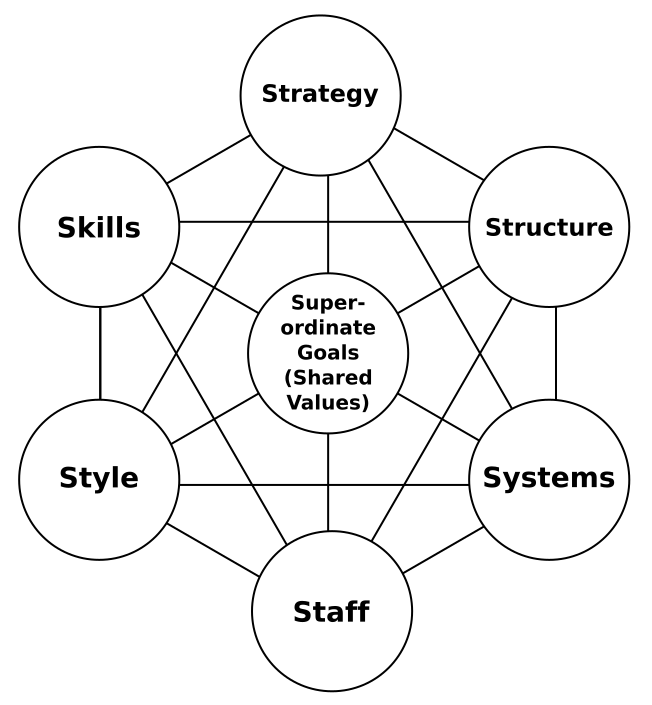
\includegraphics[width=0.6\textwidth]{graphics/sevens_framework}
    \caption{The 7S framework}
    \label{fig:sevens_framework}
\end{figure}

The model emphasises the interdependence of the factors using the connections between them. One factor may influence others, and all of them must be aligned in order for an organisation to be well organised. Also, the model is deliberately shaped in a way that does not communicate hierarchy because one factor is not necessarily more important than the others.

A brief explanation of the seven factors in terms of what question(s) each factor tries to answer:
\begin{description}
    \item[Strategy] What does the organisation do to provide added value?
    \item[Skills] What are the competencies both at the organisation level and at the level of its people?
    \item[Structure] How is the organisation arranged?
    \item[Style] How do leaders operate and interact within the organisation?
    \item[Systems] What are the rules, regulations, and processes with regard to getting things done and management activities?
    \item[Staff] How does the organisation make sure it has the right people?
    \item[Shared Values] What are the core beliefs in the organisation about what is important and why the organisation exists?
\end{description}

\section{IKEA}
- required non-software company
- largest furniture retailer of the world since 2008
- known for self-assembly furniture
- interesting because world-leading company

\paragraph{Strategy}
\citep{kumar2000market}
- design: in-house as opposed to independent
- design: simple as opposed to complex
- parts: modular-interchangeable parts as opposed to high level-wip
- parts: cheap, mass production as opposed to expensive hand-made
- assembly: self-assembly as opposed to built-to-order
- transport: efficient and computerised due to mass produced modular parts as opposed to (inefficient) transport of costly, bulky finished product
- marketing: leverage Scandinavian image and cheap out-of-town display as opposed to fragmented image across geographies and expensive high-street display
- service: self-service and self-transport vs full-service and delivery

\paragraph{Systems}

\paragraph{Structure}

\paragraph{Skills}

\paragraph{Shared values}

\paragraph{Staff}

\paragraph{Style}


% START OF GOOGLE SECtiON
\section{Google}

\paragraph{Strategy}
Google's public vision is not stated clearly on their website. Other sources indicate that the following is Google's vision: ``to provide access to the world’s information in one click''\footnote{\url{http://panmore.com/google-vision-statement-mission-statement}}. Nowadays, Google is known for many services. However, one service is at the core of Google: search. Needless to say that there are still many challenges in that area. Nonetheless, Google is dedicated to keep investing in this area and explore new techniques and methods to change the status quo.

\paragraph{Systems}
In general, Google teams tend to use agile methods. Some teams adopt XP or Scrum, but there is no company guideline as to which methodology to use. Most teams are self-organising and are free to choose whatever software processes they see fit. Teams often do not even have a project manager assigned; teams communicate directly with stakeholders \citep{striebeck2006ssh}. Google's management does not want to impose methodologies on teams and overburden them. Management believes that the teams themselves know what processes would work best for them. The software process is intentionally not centralised, and a person working at Google even claims that Google's philosophy is the exact opposite of something like CMMI\footnote{\url{https://www.quora.com/What-software-development-methodology-ies-does-Google-use}} that requires certain processes to be put in place. If one team discovers that a certain practise works well for them, other teams will follow \citep{striebeck2006ssh}. Thus, there is a lot of experimentation going on at any point in time.

The AdWords team is the exception to this philosophy, in that more standards are imposed on the process employed. This is because AdWords is much more business input driven than other projects. The AdWords project does have project managers and a fairly large management team. Some projects tried to use Agile practises, but not every practice was introduced at the same time. Team members needed to become accustomed and see the benefit of a certain practice before others are introduced. Post-mortems are conducted at the end of a project, and positive and negative points of certain methodologies are reviewed in order to decide which practises should be employed in future projects. Certain practises can be modified or improved based on this feedback. Slowly, some teams that were initially reluctant to adopt formal software processes saw the value of using certain Agile practises.

Peer reviewing is required for all code written\footnote{\url{http://steve-yegge.blogspot.nl/2006/09/good-agile-bad-agile_27.html}}. When it comes to writing code, engineers are very disciplined. The result is that the whole codebase looks the same, so it's easier for people to switch teams.

\paragraph{Structure}
The organisational structure of Google can be classified as a matrix organisation, although it is one with a rather flat hierarchy. Teams are assigned by function and by product. For example, a web developer is assigned to the Engineering \& Design\footnote{\url{https://www.google.com/about/careers/teams/}} team, as well as the Google+ team. Google's organisational structure is relatively flat. That is, there hardly is any middle management and the upper management can be approached quite easily.

\paragraph{Skills}
In the past, Google, as a company, excelled in quick decision making. When Larry Page took over as CEO in 2012 and reformed decision making at the company\footnote{\url{https://www.thinkwithgoogle.com/articles/start-up-speed-kristen-gil.html}}, he believed that as the company had grown, it had become less agile\footnote{\url{http://michael-roberto.blogspot.nl/2012/01/larry-page-reforms-decision-making-at.html}}. Another area of competence is the ability to provide more relevant search results than its competitors, particularly because of the development of the PageRank algorithm.

\paragraph{Shared values}
As of 2016, Google has the following mission: "to organise the world’s information and make it universally accessible and useful."\footnote{\url{https://www.google.com/intl/en/about/}}. Google encourages risk taking, non-traditional thinking, and innovation by employees\footnote{\url{http://2012books.lardbucket.org/books/an-introduction-to-organizational-behavior-v1.1/s15-01-decision-making-culture-the-ca.html}}. In addition, Google deeply values integrity, collaboration, and trust \citep{striebeck2006ssh}. The following quote conveys those shared values: "When a vice president in charge of the company’s advertising system made a mistake costing the company millions of dollars and apologised for the mistake, she was commended by Larry Page, who congratulated her for making the mistake and noting that he would rather run a company where they are moving quickly and doing too much, as opposed to being too cautious and doing too little."\footnote{\url{https://www.linkedin.com/pulse/20140904061228-154884582-organizational-culture-in-google-inc}}. Thus, making mistakes is accepted, and agility is a shared value. This has consequences for the software processes in place at the company. After all, a new process, such as Scrum, may be experimented with on a small scale to see if it works out and the rest of the company should adopt it. This is also why Google allows employees to spend 20\% of their time on their own ideas.
Founder Sergey Brin states that the company's culture should not be static; it should continuously improve. This may facilitate adoption of new software processes. Google has even appointed a 'chief culture officer' to guide this.

\paragraph{Staff}
Google's hiring policy is that they only recruit the brightest and best individuals. In terms of Etzioni's compliance theory\citep{lunenburg2013compliance}, Google can be classified as being a Normative-Moral organisation when considering the type of power they use to direct the behaviour of their members and the type of involvement of the participants. Normative because most employees share the vision to innovate and passion for the company to succeed and change the state of technology. Moral because employees are proud to work at Google and are often loyal to the company, staying with the company for years at end.

\paragraph{Style}
It is publicly known that Google values decisions made by teams\footnote{\url{https://www.linkedin.com/pulse/20140904061228-154884582-organizational-culture-in-google-inc}}, as opposed to decision making by single individuals. Until recently, high-level decisions were made consensually by founders Larry Page and Sergey Brin, accompanied by CEO Eric Schmidt. Google does not enforce decision making in a top-down way. Rather, it stresses the importance of rational persuasion, and teams may propagate these decisions bottom-up. Amit Singh (Google's senior vice-president and head for worldwide enterprise services) states: "We believe in bottoms-up decision making"\footnote{\url{http://articles.economictimes.indiatimes.com/2013-12-24/news/45540233_1_chrome-os-chromebooks-hangouts}}. It is also believed that top-down decision making leads to organisational anarchy. The emphasis here is on rational, thus every decision should involve proper argumentation and should not be based on instinct or feeling.

Employees at Google usually work in open office environments. The reason behind this is the conviction that open offices foster teamwork.

% END OF GOOGLE SECTION

\section{Lessons learned}
From Google's approach we can learn that in some cases it works great to give autonomy to teams. But active experimentation is valuable too, because only then will people notice if something makes a difference or not. It also shows us that a bottom-up approach works in the case of a technological company.

\subsection{RUP}

\subsection{SCRUM}

\subsection{Failed Case}

\section{Conclusion}
\chapter{POWER}

\section{Empowerment in ?}
% What if you empower employees to make decisions regarding the continuation of a project?

\section{Conclusion}
%\chapter{Conclusion}

\bibliographystyle{plainnat}
\bibliography{references}
\begin{appendices}
    \chapter{Group Process}
\section{Methodology}
We altered our methodology on \date{16-02-2016}. We changed from the \ac{spa} to a system more resembling anarchy.
We kept the \ac{po} and \ac{ac} concepts in order to maintain some control, the product owner focuses on what is required to be in the document, the agile coach has a focus on facilitating and monitoring the process.

The reason for this was that we have found it harder to make a good 'team split' for this assignment. Additionally it seems that team members trust each other better to do their work, making the somewhat more free model more comfortable.

\section{Retrospective Previous Assignment}
Before we started on this assignment we have done a SCRUM-style retrospective on the previous assignment: listing `things we have done well' and `things we can do better'.
The items identified are listed listed in table~\ref{tab:ass1retro}.

\begin{table}[!ht]
    \centering
    \begin{tabular}{L{0,45\textwidth}L{0,45\textwidth}}
         \textbf{What did we do well?} & \textbf{What can we do better?}\\
         \midrule
            Free coffee                         & More work on Monday/Tuesday  \\ 
            Initiative \& commitment of group   & Consistency of references \\
            Topic Separation                    & Merging early / continuous integration  \\
            QA (specifically: grammar)          & Plan for document structure  \\
                                                & Structured meetings  \\
                                                & ``Always have a deliverable''  \\
                                                & Double reviewing  \\
                                                & Keeping Trello up to date. \\
    \end{tabular}
    \caption{Assignment 1 retrospective}
    \label{tab:ass1retro}
\end{table}

%Changed to share-latex.
%dont know if this still applies, as I've seen that you can check the changes. Reviewing is a bit harder though
%- Accountability vs. continuous integration trade-off 

\section{Tools}
For this assignment we use the same issue tracking tool as the previous one: Trello. It has worked well during the previous assignment and we expect that it will do so again, especially if team members implement the suggestion from the retrospective.

To fix our issue with reference consistency we switched to LaTeX for the document. LaTeX has a mature reference management system that is easy to use.
For the previous assignment Google docs was used. Luckily a similar platform exists for creating TeX files: ShareLaTeX\footnote{\url{www.sharelatex.com}}.
Like Google docs it allows for multiple people to collaborate on the same file, including an edit history.

Additionally, LaTeX facilitates early merging of the document. 
An issue with working on a large file on Google docs is that editors may get in each others way.
In LaTeX a document can be split up in multiple files that compile to one output file (e.g.: one file per chapter), allowing multiple people to work on the same document without them getting in each other's way.

\section{Roles}
The roles of the various team members are listed in table~\ref{tab:roles}.
The product owner and agile coach roles have been moved to allow different members to experience working in these roles.
In addition to that a separate Document Owner is assigned, requirement for this was that the person had to be experienced with LaTeX. 

\begin{table}[!ht]
    \centering
    \begin{tabular}{>{\bfseries}l l}
    Person                      & Roles\\
    \midrule
    Jelle van Assema            & Team Member                   \\ 
    Felix Barten                & Team Member                   \\
    Robert Diebels              & Team member, Product Owner                 \\   
    Jasper Dijt                 & Team Member, Agile Coach, Document Owner   \\
    Yoan-Alexander Grigorov     & Team Member                   \\
    Guido Loupias               & Team Member                   \\
    Edward Poot                 & Team Member                   \\
    Theologos Zacharopoulos     & Team Member                   \\
    \end{tabular}
    \caption{Role division for assignment 2}
    \label{tab:roles}
\end{table}

%\section{Task Creation}
%%Don't know if this is relevant so I'm just putting it in here
%%Not very I guess, kindof merged it with 'Task Division'.
%We decided to create tasks based solely on the deliver-ables which are expect.
%
%\textbf{Rationale:} This decision was taken in an effort to eliminate waste from the process.

\section{Task Division}
We decided to divide the tasks based on who ever would want to take them. This resembles Anarchy as we get to decide what we want to do. Possibly influences the end result.
Tasks are based on the basic layout of the document, in a `fill in the gaps' way.

A possible problem of this approach is Cherry-Picking by team members, the \ac{po} and \ac{ac} will monitor for this behaviour.

\section{Task Principles}
% These are my own ideas and I received little feedback on them. However I'll list them here.
These principle are based on several sessions of feedback we received from our lecturers.
Our lectures stressed that \emph{insights} and \emph{depth of knowledge} are the aspects of this course that contain its essence. We list the following principles for execution of tasks and use them where applicable:
\begin{compactenum}
  \item \textbf{Insights considering:}
  \begin{compactenum}
    \item What the organisation learned
    \item What we have learned
  \end{compactenum}
  \item \textbf{Depth:}
  \begin{compactenum}
    \item \textbf{Critical thinking:}
    \begin{compactdesc}
      \item[What:] Describe the problem context.
      \item[Why:] Describe why something solves the problem.
      \item[How:] Describe how the problem is solved.?
      \item[When:] Describe the  context in which the problem is solved.
    \end{compactdesc}
    \item \textbf{Balance:} Demonstrate that we have a balanced view of the subject.
  \end{compactenum}
\end{compactenum}
    \printglossary[type=\acronymtype]
    \printglossary
\end{appendices}
\end{document}
